\documentclass{packages/sysuthesis} % 默认使用电子版（不填充空白页）。如果需要双面打印版，请注释掉本行并启用下一行
\usepackage{packages/sysucode}  % 在论文中使用代码
\usepackage{xurl}
\usepackage[most]{tcolorbox} % 支持附录中的问答彩色框
\pgfplotsset{compat=1.18,compat/show suggested version=false} % 固定兼容版本并关闭提示信息
\setlength{\headheight}{13pt} % 消除 fancyhdr 的 headheight 告警
\covertitlefirst{编译原理}
\covertitlesecond{实验课第四次作业}
\ctitle{编译原理——实验第四次作业}
\cauthor{林宏宇}   
\studentid{23320093}
\cschool{计算机学院}
\cmajor{计算机科学与技术}
\emajor{Computer Science and Technology}
\cmentor{李文军}
     % 论文相关信息
% 中文
\cabstract{
根据实验内容 \cite{lab04}, 在此次实验需要实现一个基于 Java 的表达式计算器，此报告参照评分标准\cite{labeval04}，完成这份实验报告撰写并附上相应的实验报告说明。

本实验设计并实现了完整的编译器前端系统，包括：（1）词法分析器，能够识别 Pascal 风格数值常量（含科学记数法）、布尔常量、预定义函数名与各类运算符，并对非法词法单元进行精确错误检测；（2）基于 11 级优先级的算符优先语法分析器，正确处理一元取负与二元减法的重载消歧义、幂运算和三元运算的右结合性、预定义函数的可变参数；（3）严格的语义处理程序，通过类型推导机制实现类型兼容性检查，确保布尔值不参与算术运算、数值值不参与逻辑运算。本实验共编写了 49 个自定义扩展测试用例，综合覆盖 simple.xml、standard.xml 和 mytest.xml 三套测试集全部 73 个用例，通过率均为 100\%，并生成了完整的 javadoc 文档。此报告详细阐述了二义性分析、词法分析、优先级表构造、语法分析与语义处理的设计与实现，并报告了实验结果与工程实践成果。
}

\ckeywords{编译原理；表达式计算}     % 摘要内容

\begin{document}

\frontmatter
\pagenumbering{Roman}
\makeUndergraduateCover    

\makecabstract                       
\newpage
\maketableofcontents        
\mainmatter

\definecolor{codebg}{RGB}{248,249,250}
\definecolor{codeframe}{RGB}{220,223,228}
\definecolor{codekw}{RGB}{25,85,145}
\definecolor{codecm}{RGB}{90,125,90}
\definecolor{codestr}{RGB}{136,44,136}
\lstdefinestyle{cleanjava}{
  language=Java,
  basicstyle=\ttfamily\small,
  keywordstyle=\bfseries\color{codekw},
  commentstyle=\itshape\color{codecm},
  stringstyle=\color{codestr},
  backgroundcolor=\color{codebg},
  frame=single,
  rulecolor=\color{codeframe},
  framesep=6pt,
  numbers=left,
  numberstyle=\scriptsize\color{gray},
  numbersep=8pt,
  breaklines=true,
  breakatwhitespace=false,
  showstringspaces=false,
  keepspaces=true,
  tabsize=4,
  columns=fullflexible
}


\chapter{实验目的}
本实验旨在设计并实现一个基于表达式的计算器 \textbf{ExprEval}，通过完整的词法分析、算符优先语法分析（Operator Precedence Parsing, OPP）和语义处理，深入理解和掌握编译原理中的核心技术。主要目标包括：
\begin{itemize}
  \item \textbf{词法分析程序的设计与实现}：根据表达式语言的词法规则，构造有限状态自动机作为程序蓝图，识别 Pascal 风格的数值常量（含科学记数法）、布尔常量、预定义函数名、各类运算符等，并对非法词法单元进行精确的错误检测与分类。
  \item \textbf{算符优先分析技术}：构造包含 11 级优先级的算符优先关系表，处理重载的一元/二元运算符（如一元取负与二元减法）、三元运算符（?:）、预定义函数等，正确处理左结合与右结合性质。
  \item \textbf{语义处理技术}：完成类型推导与类型兼容性检查，正确区分数值类型和布尔类型的子表达式，检测除数为零等运行时语义错误。
  \item \textbf{面向对象设计与软件工程实践}：采用面向对象风格设计类结构，编写 javadoc 文档化注释，编写自定义测试用例并通过实验软装置完成回归测试。
\end{itemize}


\chapter{项目组织}
\begin{itemize}
  \item \textbf{src/parser/}：源代码目录。
    \begin{itemize}
    \item \texttt{Calculator.java}：表达式计算器的核心实现，包含词法分析器（Lexer）、算符优先语法分析器（Parser）和语义处理程序（Evaluator）的全部代码。
    \end{itemize}
  \item \textbf{bin/}：编译生成的字节码目录。
    \begin{itemize}
    \item \texttt{bin/parser/}：Calculator 编译后的 class 文件。
    \item \texttt{bin/exceptions/}：实验软装置预定义的 16 种异常类。
    \item \texttt{bin/gui/}：GUI 主窗口及其内部类（预编译）。
    \item \texttt{bin/test/}：自动回归测试程序（预编译）。
    \end{itemize}
  \item \textbf{doc/}：javadoc 生成的 HTML 格式设计文档。
  \item \textbf{testcases/}：测试用例 XML 文档目录。
    \begin{itemize}
    \item \texttt{simple.xml}：简单测试用例（8 个）。
    \item \texttt{standard.xml}：标准测试用例（16 个，覆盖所有简单用例）。
    \item \texttt{mytest.xml}：自定义扩展测试用例（49 个，覆盖边缘情况）。
    \end{itemize}
  \item \textbf{build.bat / Makefile}：Windows batch 脚本和跨平台 Makefile，支持构建、测试、运行与文档生成。
\end{itemize}


\chapter{实验实现}

\section{语法定义的二义性分析}

根据实验规格说明中给出的 BNF 定义（第 2.3.1 节），ExprEval 所支持的表达式语言存在二义性。

\textbf{二义性来源分析}：

\begin{enumerate}
    \item \textbf{一元取负与二元减法运算符的重载}：BNF 中一元取负 $-$ ArithExpr 与二元减法 ArithExpr $-$ ArithExpr 使用了相同的终结符 ``$-$''。对于输入 ``$2 - 3 * -4$''，减号既可以被解释为一元取负（$-4$），也可以被解释为二元减法（$2 - 3$ 与某个表达式的差）。这种重载导致语法分析器需要通过上下文来判定减号的真实含义。

    \item \textbf{三元运算符 $?:$ 的嵌套}：BNF 中 BoolExpr ? ArithExpr : ArithExpr 是一个右结合的产生式。对于 ``$a\ ?\ b\ ?\ c\ :\ d\ :\ e$''，如果不规定结合性，既可以理解为 $a\ ?\ (b\ ?\ c\ :\ d)\ :\ e$（右结合），也可以理解为 $(a\ ?\ b\ ?\ c\ :\ d)\ :\ e$（错误解析）。若语法未明确结合性质，则存在二义性。

    \item \textbf{布尔表达式与算术表达式的上下文依赖}：BoolExpr 和 ArithExpr 在 BNF 中相互引用。例如 BoolExpr 可推导出 ArithExpr $>$ ArithExpr，而 ArithExpr 又可包含 BoolExpr ? ArithExpr : ArithExpr。这种交叉引用在纯 BNF 层面构成间接二义性，因为比较运算的结果（布尔类型）在语法层面并未与算术运算的输入（数值类型）作出区分，需要借助语义分析中的类型推导来分辨合法与非法表达式。
\end{enumerate}

\textbf{二义性的消除}：

本实验通过算符优先分析技术消除二义性：
\begin{itemize}
    \item \textbf{一元取负与二元减法}：通过上下文状态标志 \texttt{expectOpnd} 来区分。当语法分析器期望一个运算量时，遇到的 ``$-$'' 识别为一元取负；当期望一个运算符时，遇到的 ``$-$'' 识别为二元减法。一元取负具有比二元减法（以及幂运算）更高的优先级（级别 9），确保了 ``$-3^2$'' 被解析为 $(-3)^2$ 而非 $-(3^2)$。

    \item \textbf{三元运算符嵌套}：明确规定 $?:$ 为右结合，并在算符优先关系表中通过右结合的处理规则来实现：当栈顶运算符与当前 $?$ 优先级相同时，不归约栈顶，而是将新的 $?$ 压栈，从而保证右侧的 $?:$ 优先配对。

    \item \textbf{类型二义性}：在语义处理阶段通过类型检查机制解决。本实验使用 \texttt{Val} 内部类记录了每个值的类型（\texttt{isBool} 字段），在归约时检查操作数类型与运算符的兼容性，对不兼容的组合抛出 \texttt{TypeMismatchedException}。
\end{itemize}

\section{词法分析程序的设计与实现}

\subsection{词法规则}

ExprEval 所支持表达式语言的词法规则如下：

\begin{itemize}
    \item \textbf{空白符号}：仅使用空格（Space）作为单词分隔符，多个连续空格视为单个分隔。制表符、回车、换行、注释等均不允许出现。

    \item \textbf{数值类型常量}：支持 Pascal 风格的无符号数值常量，符合以下正则定义：
    \begin{align*}
        \textit{digit} &\rightarrow 0|1|2|3|4|5|6|7|8|9 \\
        \textit{integral} &\rightarrow \textit{digit}^+ \\
        \textit{fraction} &\rightarrow .\ \textit{integral} \\
        \textit{exponent} &\rightarrow (E\,|\,e)\ (+\,|\,-\ |\ \varepsilon)\ \textit{integral} \\
        \textit{decimal} &\rightarrow \textit{integral}\ (\textit{fraction}\ |\ \varepsilon)\ (\textit{exponent}\ |\ \varepsilon)
    \end{align*}
    注意：不支持负数常量（如 $-3.14$ 是数值常量 $3.14$ 的一元取负运算），小数点前后必须有数字。

    \item \textbf{布尔类型常量}：仅允许 \texttt{true} 和 \texttt{false}，大小写无关。

    \item \textbf{预定义函数名}：\texttt{sin}、\texttt{cos}、\texttt{max}、\texttt{min}，大小写无关。

    \item \textbf{运算符}：包括算术运算符（\texttt{+ - * / \^{}}）、关系运算符（\texttt{= <> < <= > >=}）、逻辑运算符（\texttt{\& | !}）、三元运算符（\texttt{? :}）、括号和逗号。
\end{itemize}

\subsection{词法分析实现}

词法分析程序嵌入在 \texttt{Calculator} 类中，核心方法为 \texttt{lex()}。该方法逐字符扫描输入字符串，根据首字符将不同类别单词的识别分派给三个私有方法：

\begin{itemize}
    \item \texttt{lexNumber()}：识别数值常量。按照上述正则定义构造识别流程：先读取整数部分（\texttt{integral}），若遇小数点则读取小数部分（\texttt{fraction}），若遇 \texttt{e/E} 则读取指数部分（\texttt{exponent}）。每一步若发现格式错误（如小数点后无数字、\texttt{E} 后无指数等），立即抛出 \texttt{IllegalDecimalException}。特别注意：以 ``.'' 开头的数值（如 \texttt{.11}）缺少整数部分，直接抛出异常；数值后若紧跟字母或额外小数点（如 \texttt{12.3Emax}、\texttt{3.3e3.3}），同样判定为非法数值常量。

    \item \texttt{lexIdent()}：识别标识符。读取连续字母序列后，在关键字表中匹配。若为 \texttt{true} 或 \texttt{false}（大小写无关），生成布尔类型 Token；若为 \texttt{sin}、\texttt{cos}、\texttt{max} 或 \texttt{min}，生成函数类型 Token；否则抛出 \texttt{IllegalIdentifierException}。例如，\texttt{mix} 导致词法错误，而 \texttt{sin5} 被正确地识别为函数名 \texttt{sin} 加上数值常量 \texttt{5}（因标识符与后续单词之间无需空白分隔）。

    \item \texttt{lexSymbol()}：识别运算符和界符。单字符运算符（\texttt{+ * / \^{} \& | ! ( ) , ? : - =}）直接匹配；双字符运算符（\texttt{<= >= <>}）在读取首字符后前瞻（lookahead）下一个字符确认。
\end{itemize}

\section{算符优先关系表的构造}

\subsection{优先级定义}

本实验按照规格说明定义了严格的 11 级优先级体系，如表~\ref{tab:prec-table} 所示。优先级数值越高表示结合越紧密。

\begin{table}[htbp]
    \centering
    \begin{tabular}{|c|c|c|c|}
    \hline
    \textbf{级别（高→低）} & \textbf{算符} & \textbf{描述} & \textbf{结合性质} \\
    \hline
    1（最紧）& \texttt{( )} & 括号 & —— \\
    2 & \texttt{sin cos max min} & 预定义函数 & —— \\
    3 & $-$（一元）& 取负运算 & 右结合 \\
    4 & \texttt{\^{}} & 求幂运算 & 右结合 \\
    5 & \texttt{* /} & 乘除运算 & 左结合 \\
    6 & \texttt{+ -} & 加减运算 & 左结合 \\
    7 & \texttt{= <> < <= > >=} & 关系运算 & 左结合 \\
    8 & \texttt{!} & 非运算 & 右结合 \\
    9 & \texttt{\&} & 与运算 & 左结合 \\
    10 & \texttt{|} & 或运算 & 左结合 \\
    11（最松）& \texttt{?:} & 选择运算 & 右结合 \\
    \hline
    \end{tabular}
    \caption{算符优先级与结合性质表}
    \label{tab:prec-table}
\end{table}

\subsection{优先级函数实现}

优先级由 \texttt{prec()} 函数实现，该函数根据具体 Token 类型和是否为一元运算符返回整型优先级值：

\begin{lstlisting}[style=cleanjava]
private static int prec(TokenType t, boolean unary) {
    if (unary && t == TokenType.MINUS) return 9;
    switch (t) {
        case QUEST: case COLON: return 1;
        case OR:               return 2;
        case AND:              return 3;
        case NOT:              return 4;
        case EQ: case NE:
        case LT: case LE:
        case GT: case GE:      return 5;
        case PLUS: case MINUS: return 6;
        case MUL: case DIV:    return 7;
        case POWER:            return 8;
        default:               return 0;
    }
}
\end{lstlisting}

\textbf{关键设计点}：
\begin{itemize}
    \item 一元取负（\texttt{unary==true \&\& t==MINUS}）返回优先级 9，高于幂运算（8），确保 ``$-3^2$'' 解析为 $(-3)^2 = 9$。
    \item 三元运算符 \texttt{?} 和 \texttt{:} 处于最低优先级 1，使得关系运算和逻辑运算的结果优先于三元选择被归约。
    \item 括号和函数调用不参与优先级比较，而是在算符栈中作为特殊的同步标记（marker）处理。
\end{itemize}

\subsection{结合性质处理}

右结合性由 \texttt{rightAssoc()} 函数判定，\texttt{\^{}} 和 \texttt{?} 为右结合。在 \texttt{evalBeforePush()} 中，对于右结合运算符，仅当栈顶优先级\textbf{严格大于}当前优先级时才归约（$pTop > pIn$），而非左结合时的 $pTop \ge pIn$：

\begin{lstlisting}[style=cleanjava]
if (rightAssoc(incoming.type)) {
    if (pTop <= pIn) break;   // 右结合：栈顶优先级 <= 当前则停止归约
} else {
    if (pTop < pIn) break;    // 左结合：栈顶优先级 <  当前则停止归约
}
\end{lstlisting}

这一设计保证了对 ``$2\ \^{}\ 4\ \^{}\ 3$'' 的正确解析：第二个 \texttt{\^{}} 入栈时，栈顶的 \texttt{\^{}} 优先级等于当前，因右结合特性停止归约，最终归约顺序为 $2\ \^{}\ (4\ \^{}\ 3)$。

\section{语法分析与语义处理程序的设计与实现}

\subsection{算符优先分析核心算法}

语法分析程序采用双栈结构的算符优先分析方法。两个核心栈分别为：
\begin{itemize}
    \item \texttt{valStack}（\texttt{Stack<Val>}）：存放运算量（数值或布尔值）。
    \item \texttt{opStack}（\texttt{Stack<OpEntry>}）：存放运算符和界符。\texttt{OpEntry} 封装了 Token、是否为一元运算符标记、以及函数调用的参数基址。
\end{itemize}

此外，三元运算符 ``?:'' 的实现使用了辅助栈 \texttt{ternStack}（\texttt{Stack<TernState>}），用于在 ``?'' 和 ``:'' 被分别归约时暂存条件和真值分支。

核心解析循环在主方法 \texttt{calculate()} 中实现。对每个 Token 进行分类处理后，使用 \texttt{expectOpnd} 布尔标志跟踪期望的下一个单词类型（运算量或运算符），以此精确检测 \texttt{MissingOperandException} 和 \texttt{MissingOperatorException}。

归约动作的核心在 \texttt{evalOp()} 中完成，其对各运算符的语义处理包括类型检查和计算：

\begin{lstlisting}[style=cleanjava]
private void evalOp(OpEntry oe) throws ExpressionException {
    Token op = oe.tok;

    // 三元 ':' 归约
    if (op.type == TokenType.COLON) {
        Val falseVal = valStack.pop();
        TernState ts = ternStack.pop();
        if (!ts.cond.isBool) throw new TypeMismatchedException();
        Val res = (ts.cond.v != 0) ? ts.trueBranch : falseVal;
        valStack.push(res);
        return;
    }
    // 一元取负
    if (op.type == TokenType.MINUS && oe.isUnary) { ... }
    // 一元逻辑非
    if (op.type == TokenType.NOT) { ... }
    // 二元运算：弹出左右操作数，类型检查，计算并压栈
    Val b = valStack.pop();
    Val a = valStack.pop();
    switch (op.type) { ... }
}
\end{lstlisting}

\subsection{重载运算符的处理}

表达式语言中存在重载的运算符 ``$-$''：它既可以是一元取负，也可以是二元减法。本实验通过 \texttt{expectOpnd} 标志进行消歧义：

\begin{lstlisting}[style=cleanjava]
case MINUS:
    if (expectOpnd) {
        opStack.push(new OpEntry(t, true));  // 一元取负
        sawComma = false;
    } else {
        evalBeforePush(t, false);             // 二元减法：先归约栈中更高优先级的运算
        opStack.push(new OpEntry(t, false));
        expectOpnd = true;
    }
    pos++;
    break;
\end{lstlisting}

当期望一个运算量时，遇到的 ``$-$'' 被识别为取负运算符并压入 opStack（标记为 \texttt{isUnary=true}）；当期望运算符时，遇到的 ``$-$'' 按二元减法处理，先归约栈顶所有优先级不低于它的运算符再入栈。

\subsection{类型推导与兼容性检查}

语义处理的核心是类型推导。\texttt{Val} 内部类通过 \texttt{isBool} 字段标记子表达式的类型。各类运算符的类型检查规则如下：

\begin{itemize}
    \item \textbf{算术运算符}（\texttt{+ - * / \^{}}）：两个操作数必须均为数值类型，结果为数值类型。
    \item \textbf{关系运算符}（\texttt{= <> < <= > >=}）：两个操作数必须均为数值类型，结果为布尔类型。
    \item \textbf{逻辑运算符}（\texttt{\& |}）：两个操作数必须均为布尔类型，结果为布尔类型。
    \item \textbf{一元逻辑非}（\texttt{!}）：操作数必须为布尔类型，结果为布尔类型。
    \item \textbf{一元取负}（$-$）：操作数必须为数值类型，结果为数值类型。
    \item \textbf{三元运算符}（\texttt{?:}）：条件必须为布尔类型，真/假分支均为数值类型，结果为数值类型。
    \item \textbf{预定义函数}：所有参数必须为数值类型，结果为数值类型。
\end{itemize}

特别地，根据规格说明第 2.4.5 节的规定，\textbf{布尔类型的值不可作为计算器最后的求值结果}。因此在 \texttt{calculate()} 方法末尾，若最终结果 \texttt{isBool} 为 \texttt{true}，则抛出 \texttt{TypeMismatchedException}。

\subsection{预定义函数的处理}

预定义函数 \texttt{sin} 和 \texttt{cos} 要求有且仅有 1 个参数；\texttt{max} 和 \texttt{min} 支持可变数目的参数，但至少需要 2 个参数。参数个数的校验规则如下：

\begin{itemize}
    \item \texttt{sin/cos}：参数个数小于 1 $\rightarrow$ \texttt{MissingOperandException}；参数个数大于 1 $\rightarrow$ \texttt{FunctionCallException}。
    \item \texttt{max/min}：参数个数小于 2 $\rightarrow$ \texttt{MissingOperandException}。
\end{itemize}

函数调用通过 \texttt{handleFunc()} 方法实现。进入函数时，\texttt{LPAREN} 的 OpEntry 记录了 \texttt{valStack} 的当前大小作为参数基址；遇到逗号时通过 \texttt{evalUntil(LPAREN)} 归约当前参数；遇到右括号时弹出参数并完成函数计算。

\subsection{三元运算符的处理}

三元运算符 ``?:'' 因其分为 ``?'' 和 ``:'' 两个独立的 Token，需要特殊的语法分析处理。本实现使用三个辅助结构与三个步骤：

\textbf{步骤一}（遇到 ``?''）：因为 ``?:'' 优先级最低，先通过 \texttt{evalBeforePush} 归约条件表达式中所有更高优先级的运算，弹出条件值并暂存于 \texttt{ternStack}，然后将 ``?'' 压入 \texttt{opStack} 作为标记。

\textbf{步骤二}（遇到 ``:''）：通过 \texttt{evalUntil(QUEST)} 归约 ``?'' 上方（真值分支）的所有运算。弹出真值，从 \texttt{ternStack} 取出对应条件，将条件与真值一并保存后，将 ``:'' 压入 \texttt{opStack} 作为待完成的标记。

\textbf{步骤三}（``:'' 归约或表达式结束）：当 ``:'' 被归约时（可能因遇到更外层的 ``:'' 或表达式末尾），弹出假值分支的结果，从 \texttt{ternStack} 取出条件与真值，完成三目选择计算并将结果压入 \texttt{valStack}。

这一设计正确处理了三元运算符的右结合嵌套。对于 ``$a\ ?\ b\ ?\ c\ :\ d\ :\ e$''，内层的 ``$b\ ?\ c\ :\ d$'' 会先在遇到第二个 ``:'' 时完成归约，得到内层结果后再与外层的条件和假值分支组合，最终等价于 $a\ ?\ (b\ ?\ c\ :\ d)\ :\ e$。

\section{自定义测试用例设计与覆盖}

本实验在完成 standard.xml 全部 16 个测试用例的基础上，额外编写了 49 个自定义扩展测试用例（mytest.xml），系统性地覆盖了规格说明中的边缘情况。测试用例分类如下：

\begin{itemize}
    \item \textbf{右结合性验证}：幂运算（$2^{4^{3}}$）、三元运算符（$\text{true}\ ?\ 5\ :\ \text{false}\ ?\ 1\ :\ 0$）。
    \item \textbf{一元取负}：$2.5 + (-2.4)$、$5 - (-2.5)$、$-3^2$（取负优先级高于幂）。
    \item \textbf{三元边界}：多余 ``:''（TrinaryOperationException）、缺少真/假值分支（MissingOperandException）、数值条件（TypeMismatchedException）、布尔分支（TypeMismatchedException）、括号/三元不匹配等。
    \item \textbf{布尔终值禁止}：\texttt{true}、\texttt{false}、比较运算结果、逻辑运算结果作为最终返回值均触发 TypeMismatchedException。
    \item \textbf{函数调用边界}：参数不足（MissingOperandException）、参数过多（FunctionCallException）、逗号边缘情况（$\text{cos}(3.14,\ )$、$\text{max}(,\ 1.8)$、$\text{max}(17,\ ,\ 87)$ 等）。
    \item \textbf{非法数值常量}：缺少小数部分（$3.\text{e}3$）、双重小数点（$3.3\text{e}3.3$）、指数中带小数点（$3.3\text{E}.3$）、缺少整数部分（$.11$）、数值后接字母（$12.3\text{Emax}$）。
    \item \textbf{非法标识符/符号}：未定义标识符（\texttt{v4}、\texttt{mix}）、非法符号（\texttt{@}）。
    \item \textbf{函数调用缺少括号}：$\text{max}5,6,8)$、$\text{sin}5,3)$ 触发 FunctionCallException。
    \item \textbf{缺少运算符/运算量}：两个括号表达式连缀、函数调用后紧跟数值。
\end{itemize}

\section{异常处理}
本实验严格按照实验软装置预定义的异常体系进行错误报告：在词法分析、语法分析与语义处理三个阶段一旦发现错误，立即抛出最具体的异常类型，避免使用过于宽泛的父类异常。词法分析阶段负责捕获非法数值、非法标识符与非法符号；语法分析阶段负责检测运算符/运算量缺失、括号不匹配、函数调用形式错误及三元运算符不匹配；语义处理阶段负责类型不匹配与除数为零等运行时语义错误。

\begin{table}[htbp]
    \centering
    \small
    \renewcommand{\arraystretch}{1.2}
    \begin{tabular}{|p{6.3cm}|p{3cm}|p{5cm}|}
    \hline
    \textbf{异常类型} & \textbf{类别} & \textbf{触发条件（典型示例）} \\
    \hline
    \texttt{ExpressionException} & 总基类 & 表达式错误基类；实现中不直接抛出，仅用于统一捕获。 \\
    \hline
    \texttt{LexicalException} & 词法错误基类 & 词法错误的父类；实现中不直接抛出，仅用于分类。 \\
    \hline
    \texttt{IllegalDecimalException} & 词法错误 & 非法数值常量（如 \texttt{.11}、\texttt{3.e3}、\texttt{7e}、\texttt{12.3Emax}）。 \\
    \hline
    \texttt{IllegalIdentifierException} & 词法错误 & 非法标识符（如 \texttt{mix}、\texttt{v4}）。 \\
    \hline
    \texttt{IllegalSymbolException} & 词法错误 & 非法符号（如 \texttt{@}）。 \\
    \hline
    \texttt{SyntacticException} & 语法错误基类 & 语法错误的父类；实现中不直接抛出，仅用于分类。 \\
    \hline
    \texttt{MissingOperatorException} & 语法错误 & 运算符缺失（如 \texttt{2 3}、\texttt{)(}、函数调用后直接跟数值）。 \\
    \hline
    \texttt{MissingOperandException} & 语法错误 & 运算量缺失（如 \texttt{2+}、\texttt{max(,1)}、\texttt{cos(3.14, )}）。 \\
    \hline
    \texttt{MissingLeftParenthesisException} & 语法错误 & 缺少左括号（如 \texttt{1+2)}）。 \\
    \hline
    \texttt{MissingRightParenthesisException} & 语法错误 & 缺少右括号（如 \texttt{(1+2}）。 \\
    \hline
    \texttt{FunctionCallException} & 语法错误 & 函数调用形式错误或参数个数过多（如 \texttt{sin(1,2)}、\texttt{max} 后直接跟数值）。 \\
    \hline
    \texttt{TrinaryOperationException} & 语法错误 & 三元运算符不匹配（如多余 ``:`` 或缺失 ``:``）。 \\
    \hline
    \texttt{EmptyExpressionException} & 语法错误 & 输入表达式为空或仅含空白符。 \\
    \hline
    \texttt{SemanticException} & 语义错误基类 & 语义错误的父类；实现中不直接抛出，仅用于分类。 \\
    \hline
    \texttt{DividedByZeroException} & 语义错误 & 除数为 0（如 \texttt{3/0} 或 \texttt{1/(2-2)}）。 \\
    \hline
    \texttt{TypeMismatchedException} & 语义错误 & 类型不匹配（布尔参与算术/数值参与逻辑、三元条件非布尔、布尔终值作为最终结果）。 \\
    \hline
    \end{tabular}
    \caption{异常处理总结表}
    \label{tab:exception-summary}
\end{table}

\section{有限状态自动机图表}
为满足实验要求，词法分析阶段以有限状态自动机（FSA）作为程序蓝图。图~\ref{fig:lexer-fsa} 分别给出了数值常量、标识符/关键字与运算符三类单词的识别自动机，其中双圆表示接受状态。运算符的单字符集合为 \texttt{+ - * / \^{} \& | ! ( ) , ? : =}，双字符运算符由 ``<'' 或 ``>'' 前缀扩展得到（\texttt{<=}、\texttt{>=}、\texttt{<>}）。

\begin{figure}[htbp]
    \centering
    \small
    \begin{subfigure}[t]{0.9\textwidth}
        \centering
        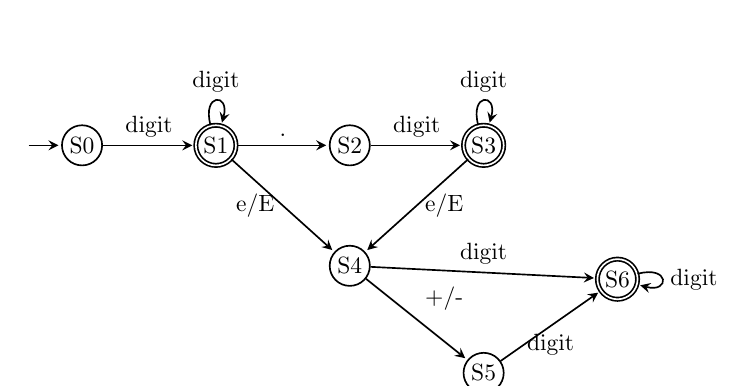
\begin{tikzpicture}[->,>=stealth,shorten >=1pt,auto,semithick,scale=0.85, every node/.style={scale=0.85}]
            \node[circle,draw,minimum size=6mm,inner sep=0pt] (s0) at (0,0) {S0};
            \node[circle,draw,double,minimum size=6mm,inner sep=0pt] (s1) at (2,0) {S1};
            \node[circle,draw,minimum size=6mm,inner sep=0pt] (s2) at (4,0) {S2};
            \node[circle,draw,double,minimum size=6mm,inner sep=0pt] (s3) at (6,0) {S3};
            \node[circle,draw,minimum size=6mm,inner sep=0pt] (s4) at (4,-1.8) {S4};
            \node[circle,draw,minimum size=6mm,inner sep=0pt] (s5) at (6,-3.4) {S5};
            \node[circle,draw,double,minimum size=6mm,inner sep=0pt] (s6) at (8,-2.0) {S6};

            \draw[->] (-0.8,0) -- (s0);
            \draw (s0) -- node{digit} (s1);
            \draw (s1) edge[loop above] node{digit} (s1);
            \draw (s1) -- node{.} (s2);
            \draw (s2) -- node{digit} (s3);
            \draw (s3) edge[loop above] node{digit} (s3);
            \draw (s1) -- node[left]{e/E} (s4);
            \draw (s3) -- node[right]{e/E} (s4);
            \draw (s4) -- node[above]{digit} (s6);
            \draw (s4) -- node{+/-} (s5);
            \draw (s5) -- node[below]{digit} (s6);
            \draw (s6) edge[loop right] node{digit} (s6);
        \end{tikzpicture}
        \caption{数值常量}
    \end{subfigure}

    \vspace{0.6em}

    \begin{subfigure}[t]{0.9\textwidth}
        \centering
        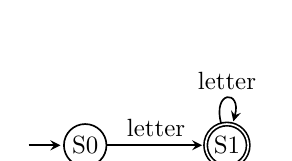
\begin{tikzpicture}[->,>=stealth,shorten >=1pt,auto,semithick,scale=0.9, every node/.style={scale=0.9}]
            \node[circle,draw,minimum size=6mm,inner sep=0pt] (s0) at (0,0) {S0};
            \node[circle,draw,double,minimum size=6mm,inner sep=0pt] (s1) at (2,0) {S1};
            \draw[->] (-0.8,0) -- (s0);
            \draw (s0) -- node{letter} (s1);
            \draw (s1) edge[loop above] node{letter} (s1);
        \end{tikzpicture}
        \caption{标识符/关键字}
    \end{subfigure}

    \vspace{0.6em}

    \begin{subfigure}[t]{0.9\textwidth}
        \centering
        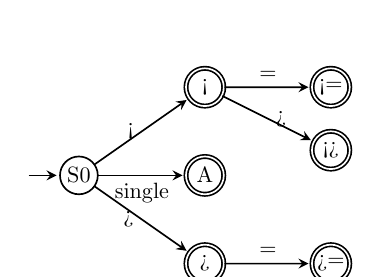
\begin{tikzpicture}[->,>=stealth,shorten >=1pt,auto,semithick,scale=0.8, every node/.style={scale=0.8}]
            \node[circle,draw,minimum size=6mm,inner sep=0pt] (s0) at (0,0) {S0};
            \node[circle,draw,double,minimum size=6mm,inner sep=0pt] (sa) at (2,0) {A};
            \node[circle,draw,double,minimum size=6mm,inner sep=0pt] (sl) at (2,1.4) {<};
            \node[circle,draw,double,minimum size=6mm,inner sep=0pt] (sg) at (2,-1.4) {>};
            \node[circle,draw,double,minimum size=6mm,inner sep=0pt] (sle) at (4,1.4) {<=};
            \node[circle,draw,double,minimum size=6mm,inner sep=0pt] (sne) at (4,0.4) {<>};
            \node[circle,draw,double,minimum size=6mm,inner sep=0pt] (sge) at (4,-1.4) {>=};

            \draw[->] (-0.8,0) -- (s0);
            \draw (s0) -- node[below]{single} (sa);
            \draw (s0) -- node[left]{<} (sl);
            \draw (s0) -- node[left]{>} (sg);
            \draw (sl) -- node{=} (sle);
            \draw (sl) -- node[right]{>} (sne);
            \draw (sg) -- node{=} (sge);
        \end{tikzpicture}
        \caption{运算符与界符}
    \end{subfigure}
    \caption{词法分析有限状态自动机示意}
    \label{fig:lexer-fsa}
\end{figure}



\chapter{实验结果与分析}

将 \texttt{Calculator.java} 编译后，通过实验软装置的自动回归测试工具对全部三套测试用例进行了完整测试，并使用 GUI 界面进行了手动GUI界面功能和计算功能测试。测试结果报告如下：

\begin{itemize}
    \item 编译成功：\texttt{Calculator.java} 成功编译，无编译错误或警告。
    \item GUI 界面基本功能测试：所有 GUI 的输入框、复制粘贴等各个按钮、帮助信息显示等均正常工作。
    \item 手动 GUI 测试：通过 GUI 界面进行的手动测试表明，所有功能均能正常工作，用户体验良好。
    \item javadoc 文档生成：成功生成完整的 javadoc 文档，包含所有类、方法和字段的注释信息，文档结构清晰，易于导航。
    \item 自动回归测试：三套测试用例全部通过，具体结果如下：
    \begin{itemize}
        \item \textbf{simple.xml}：8 个测试用例，8 个通过，通过率 100\%。
        \item \textbf{standard.xml}：16 个测试用例，16 个通过，通过率 100\%。
        \item \textbf{mytest.xml}：49 个自定义扩展测试用例，49 个通过，通过率 100\%。
    \end{itemize}
\end{itemize}

\section{编译结果}

\begin{figure}[htbp]
\centering
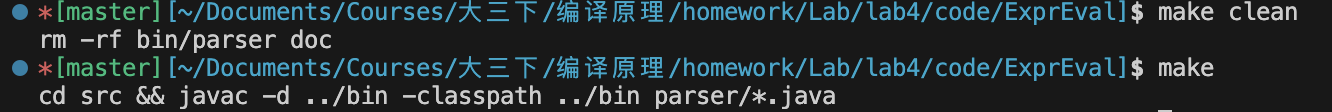
\includegraphics[width=\textwidth]{image/template/test_result/make_java.png}
\caption{编译java脚本结果截图}
\end{figure}

\begin{figure}[htbp]
\centering
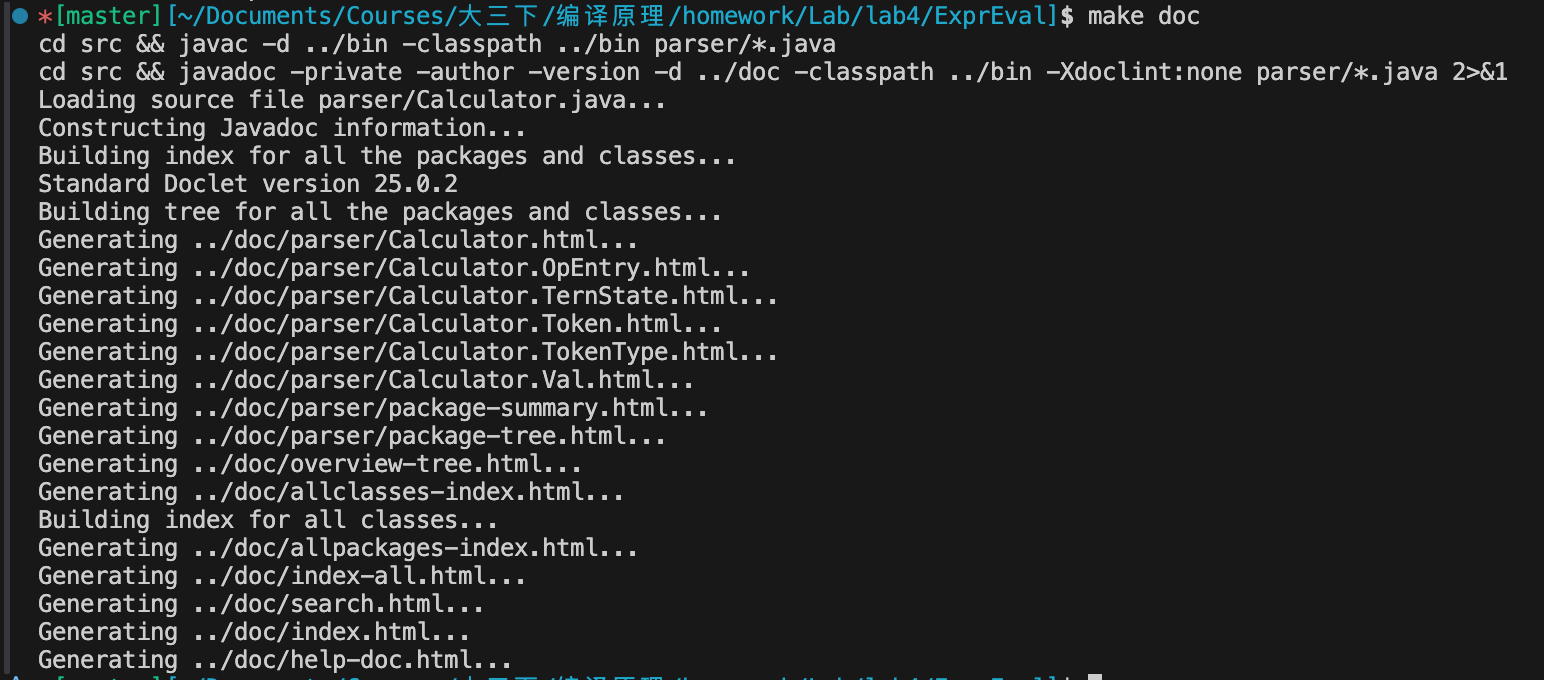
\includegraphics[width=0.8\textwidth]{image/template/test_result/make_java_doc.png}
\caption{javadoc 文档生成截图}
\end{figure}

\section{GUI界面基本功能}

\begin{figure}[htbp]
\centering
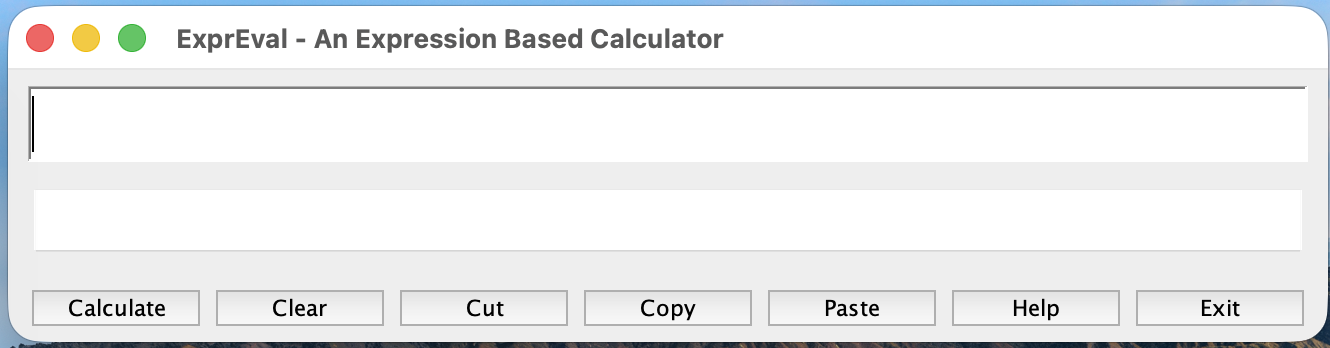
\includegraphics[width=\textwidth]{image/template/test_result/GUI1.png}
\caption{GUI 界面展示}
\end{figure}

\begin{figure}[htbp]
\centering
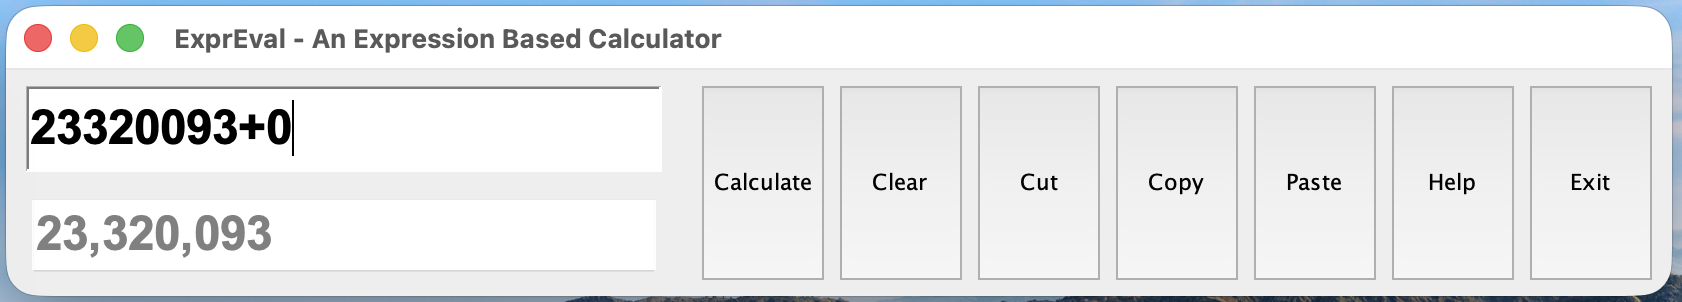
\includegraphics[width=\textwidth]{image/template/test_result/GUI2.png}
\caption{GUI 按钮移动到右方}
\end{figure}

\begin{figure}[htbp]
\centering
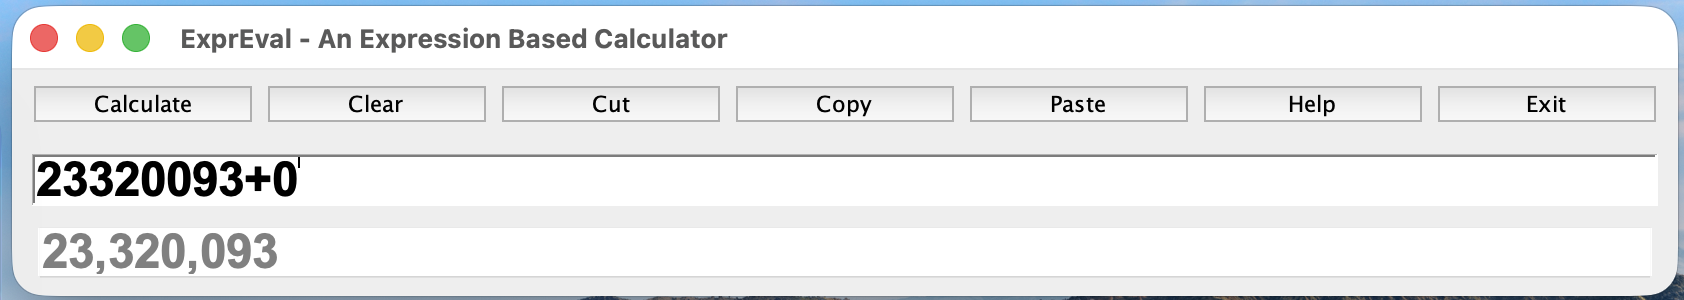
\includegraphics[width=\textwidth]{image/template/test_result/GUI3.png}
\caption{GUI 按钮移动到上方}
\end{figure}

\begin{figure}[htbp]
\centering
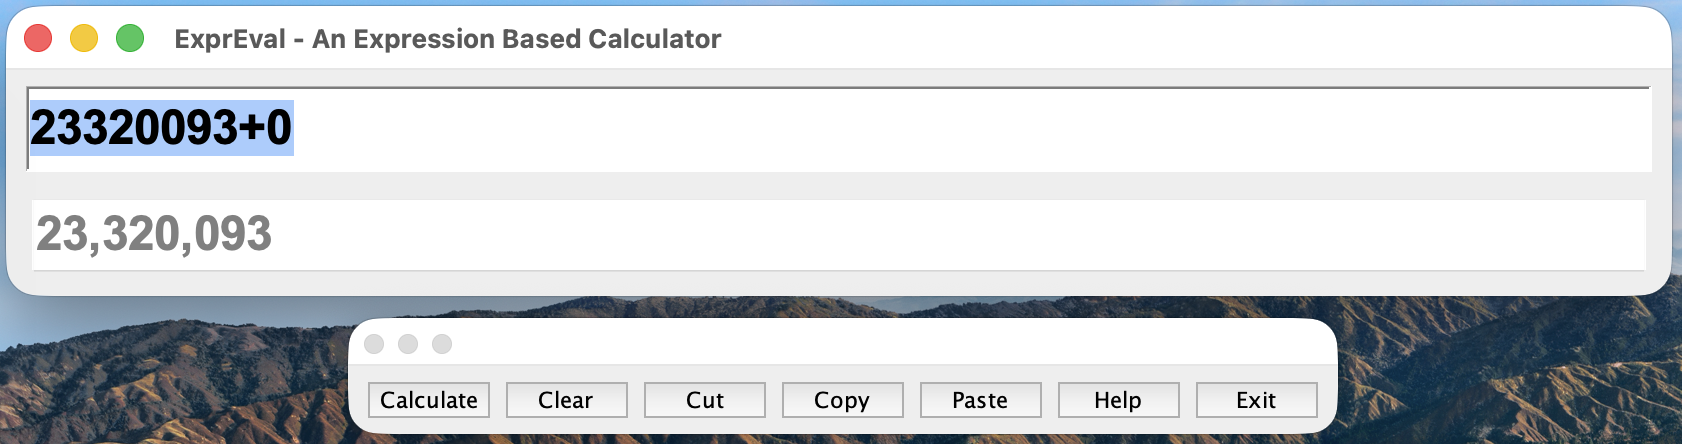
\includegraphics[width=\textwidth]{image/template/test_result/GUI4.png}
\caption{GUI 按钮移动到任意位置}
\end{figure}

\begin{figure}[htbp]
\centering
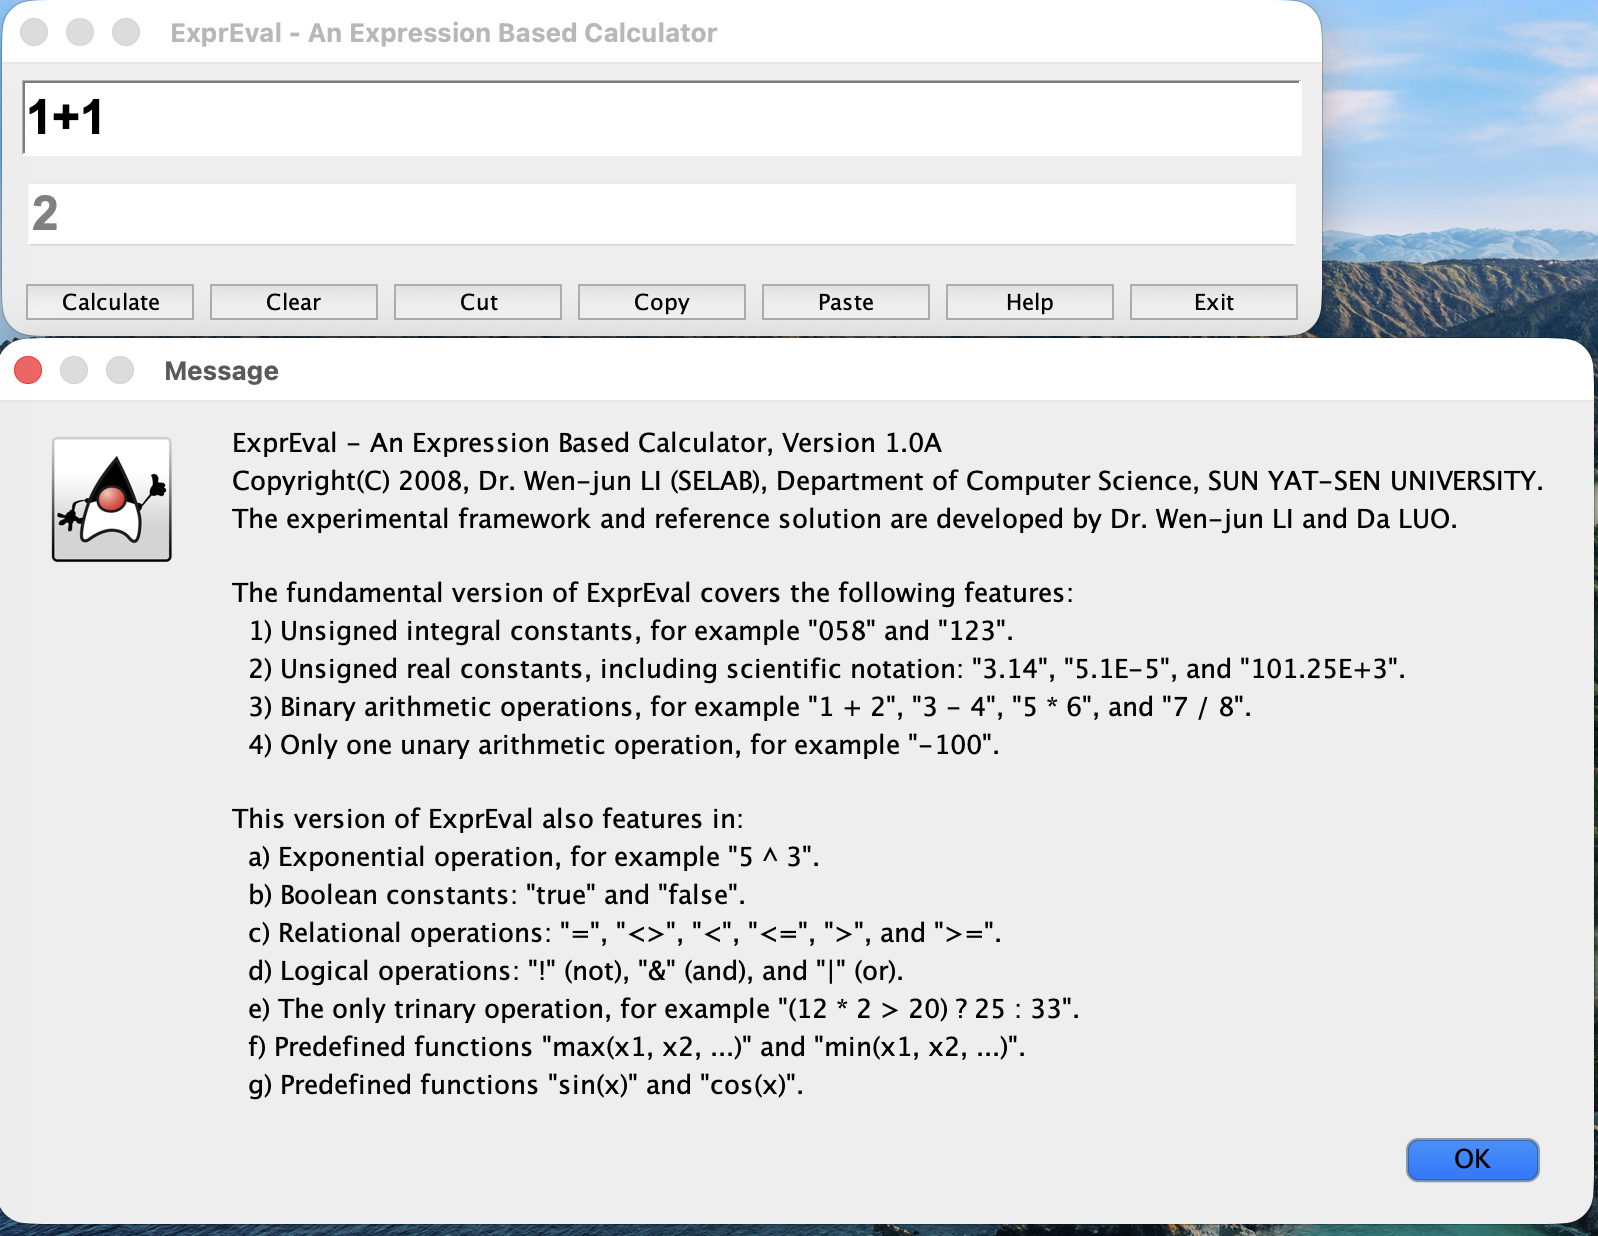
\includegraphics[width=\textwidth]{image/template/test_result/help.png}
\caption{GUI 帮助信息}
\end{figure}


\section{自动回归测试结果分析}

\begin{figure}[htbp]
\centering
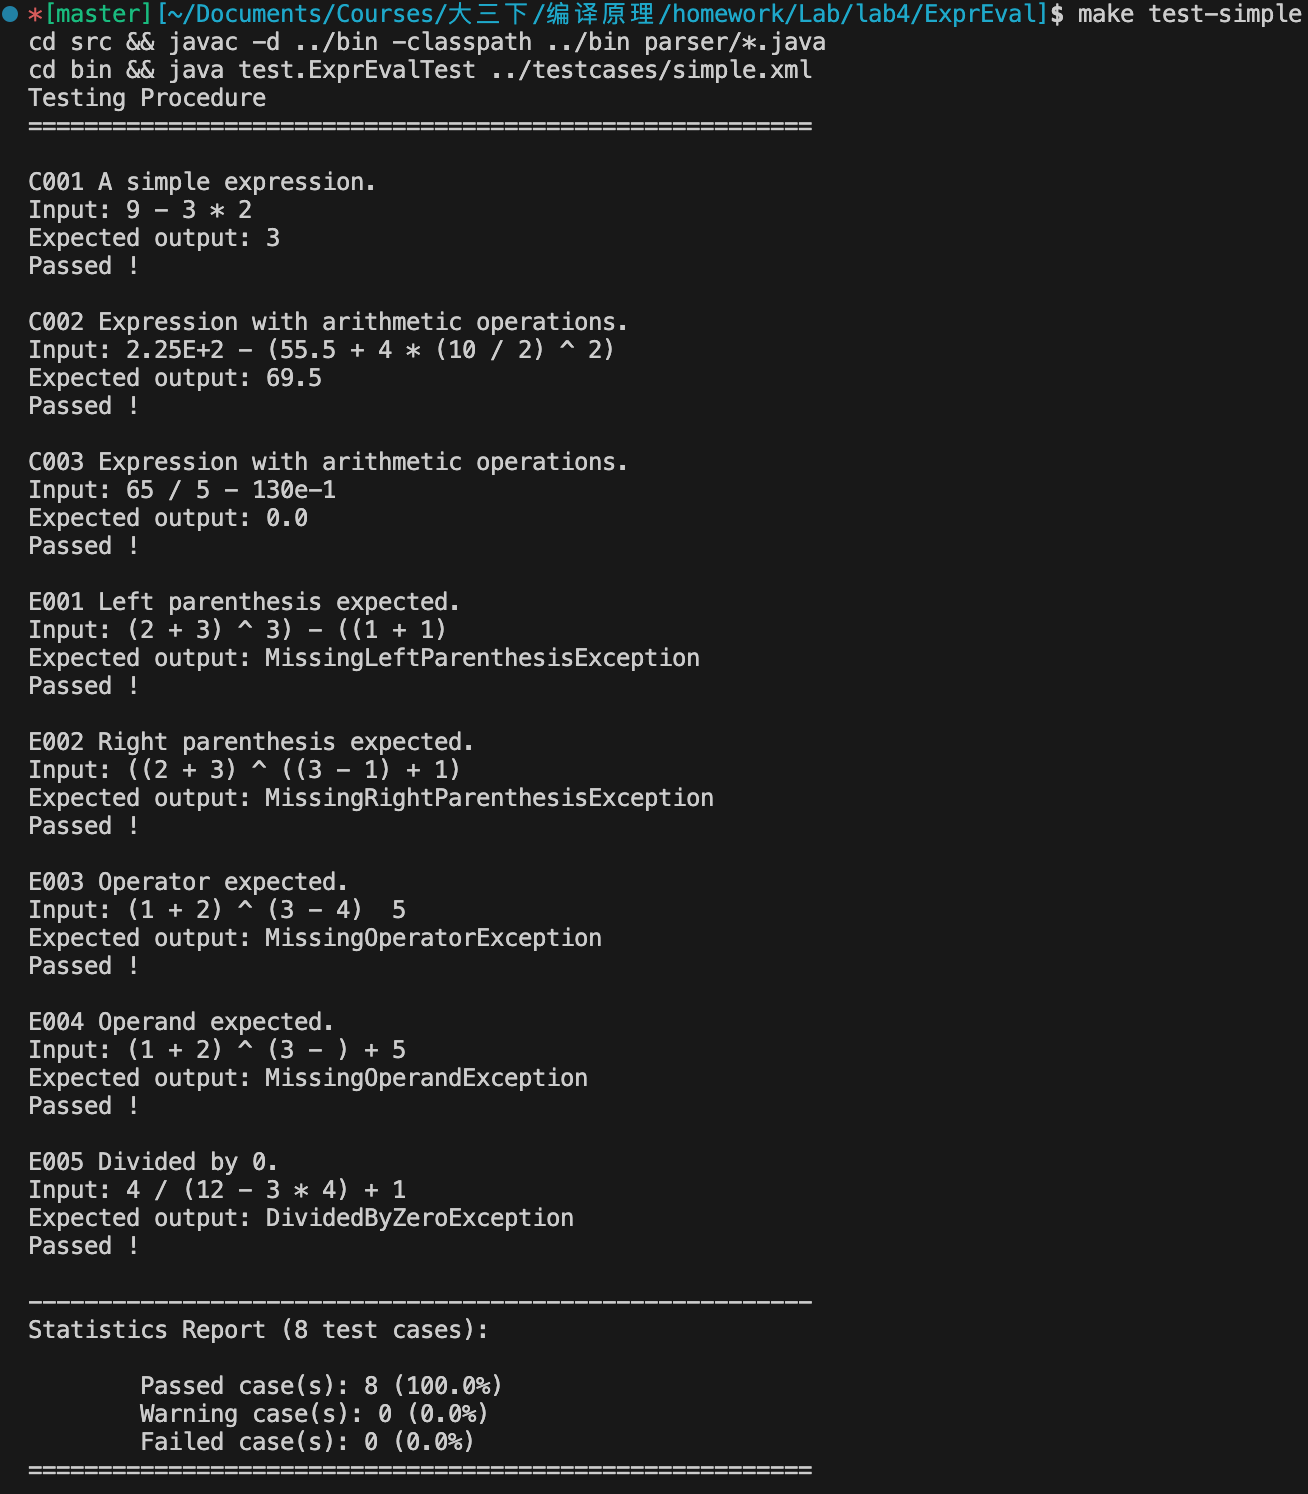
\includegraphics[width=\textwidth]{image/template/test_result/run_test_simple.png}
\caption{简单测试用例（simple.xml）运行结果截图}
\end{figure}

\begin{figure}[htbp]
\centering
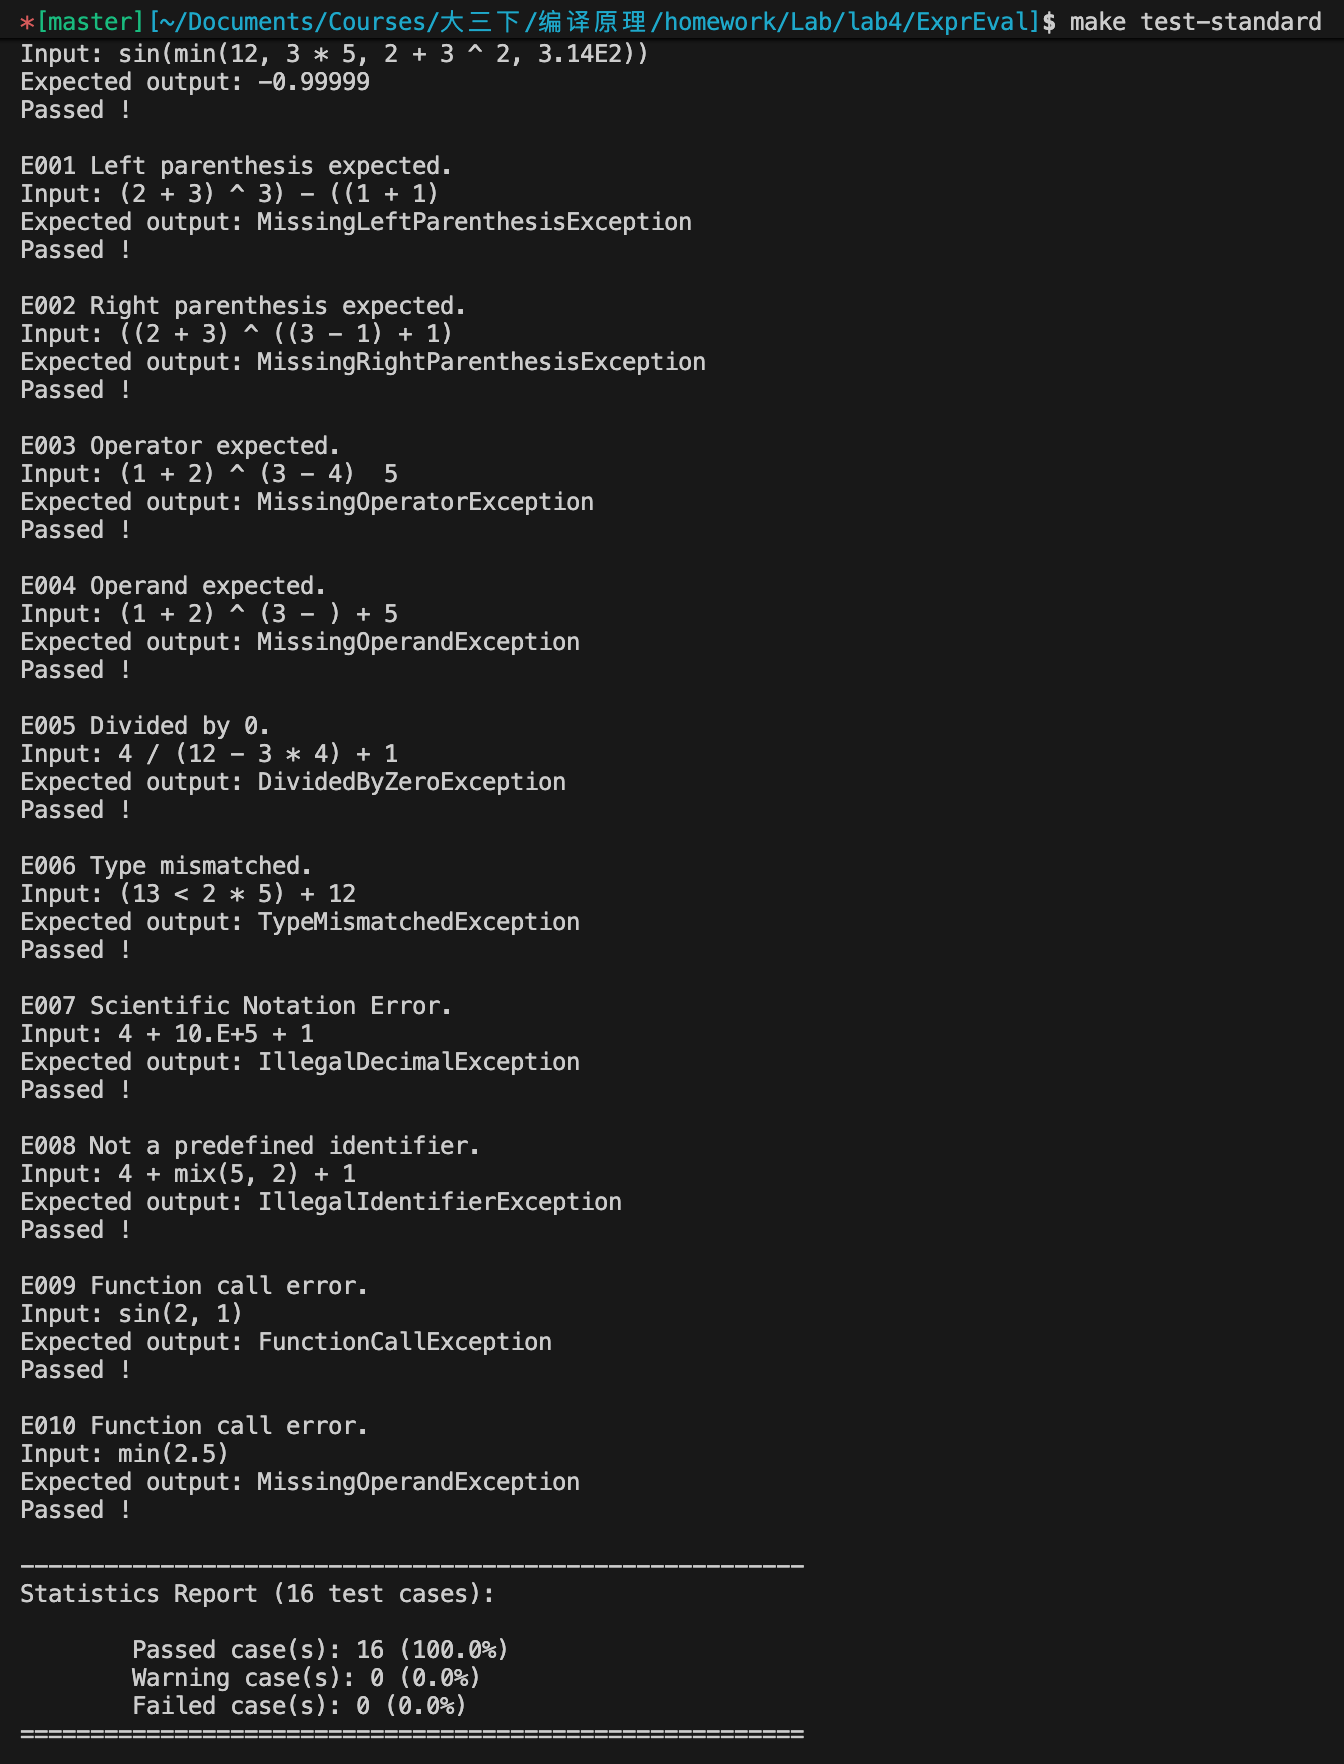
\includegraphics[width=\textwidth]{image/template/test_result/run_test_standard.png}
\caption{标准测试用例（standard.xml）运行结果截图}
\end{figure}

\begin{figure}[htbp]
\centering
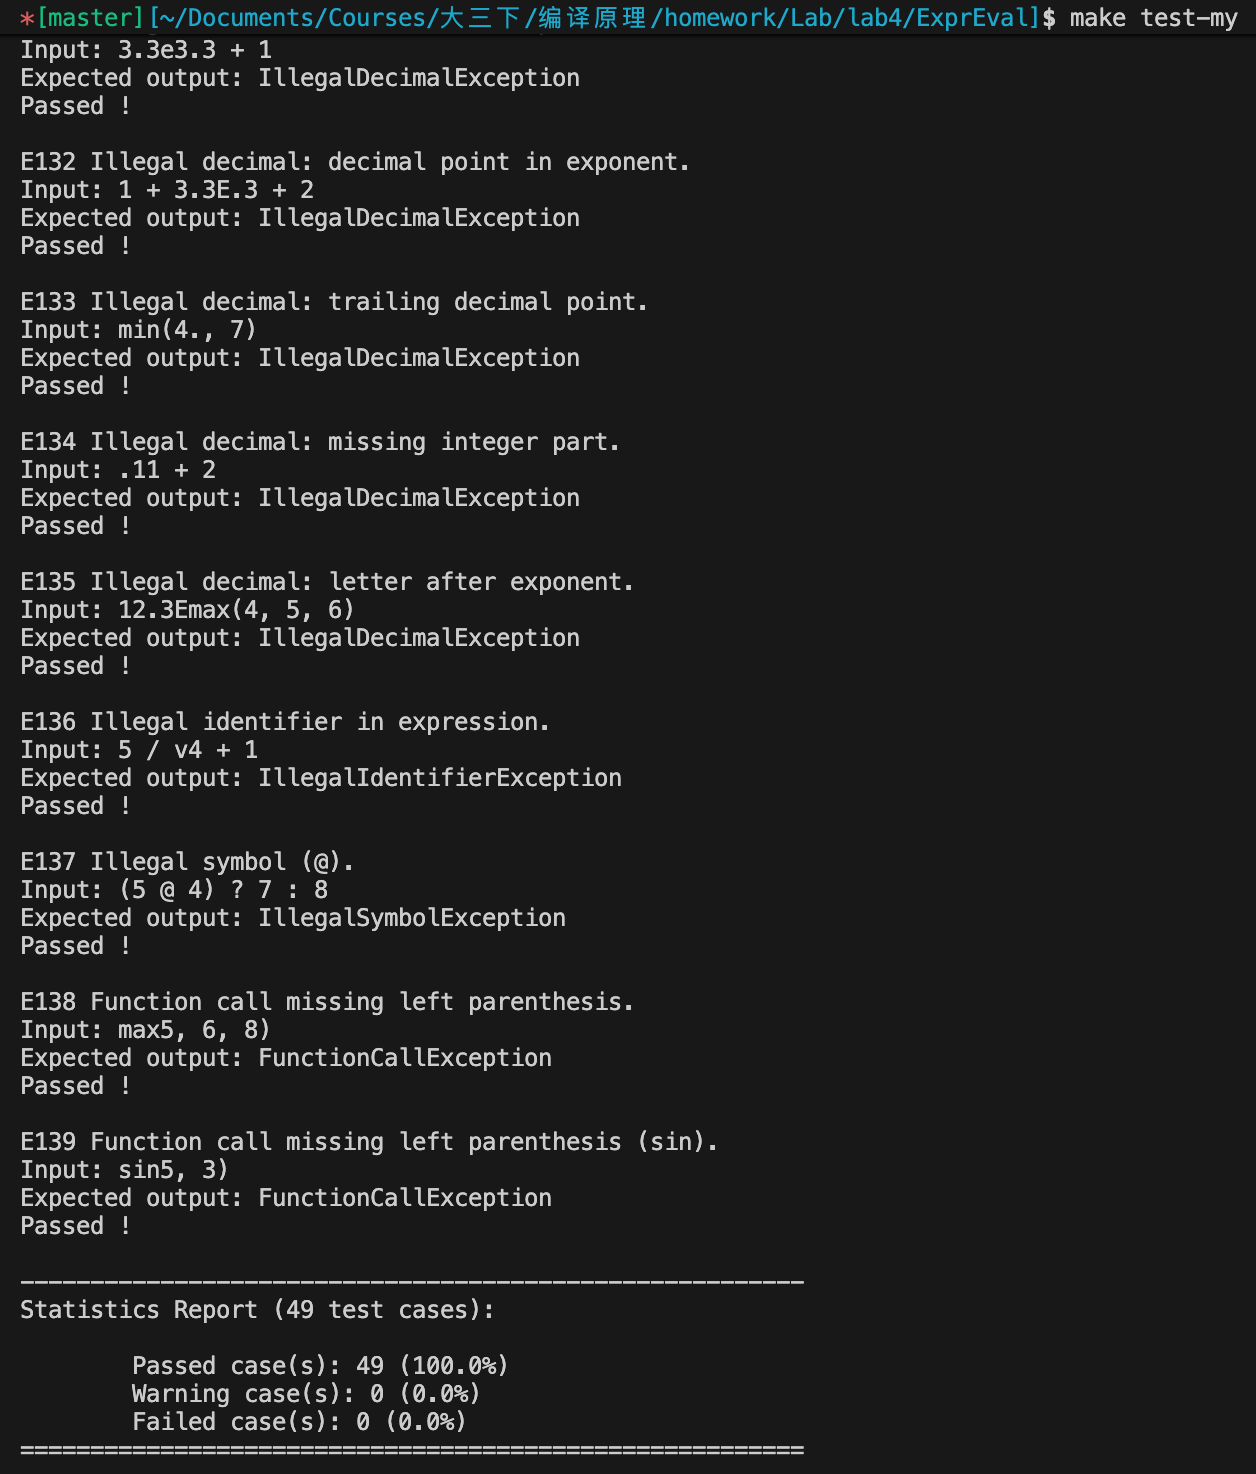
\includegraphics[width=\textwidth]{image/template/test_result/run_test_mytest.png}
\caption{自定义扩展测试用例（mytest.xml）运行结果截图}
\end{figure}


\section{手动计算测试}

由于例子实在是太多了，这里仅展示部分测试用例的计算结果截图。

\begin{figure}[htbp]
\centering
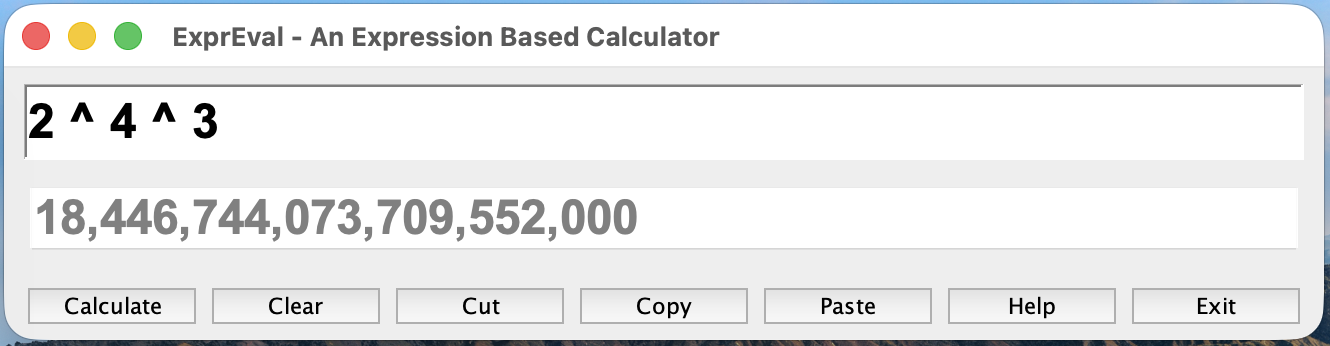
\includegraphics[width=0.7\textwidth]{image/template/test_result/calculate1.png}
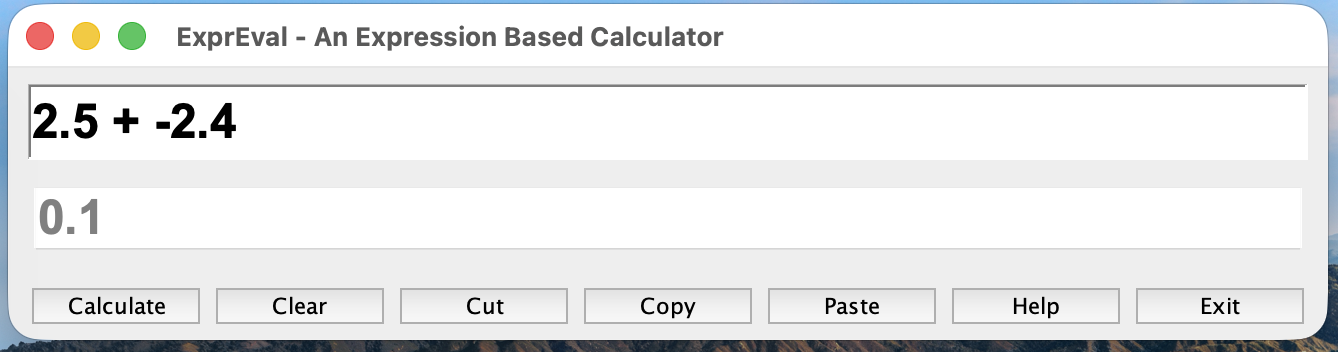
\includegraphics[width=0.7\textwidth]{image/template/test_result/calculate2.png}
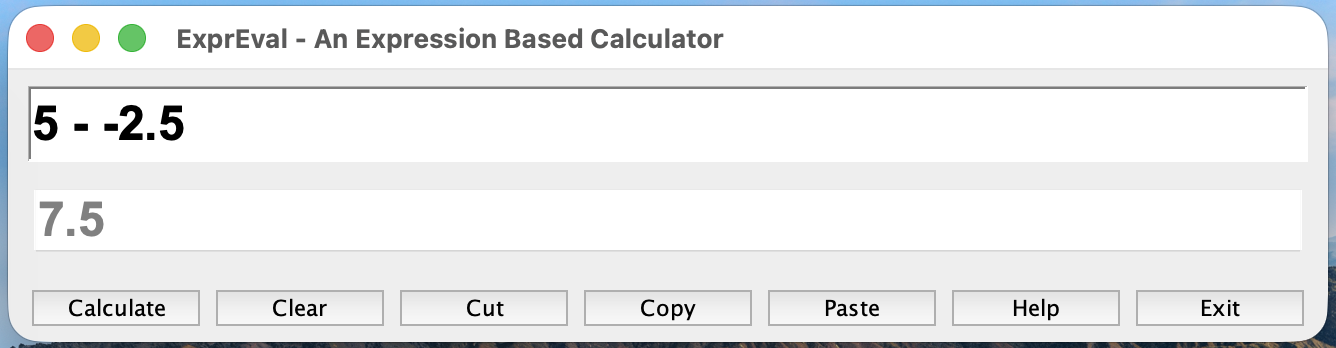
\includegraphics[width=0.7\textwidth]{image/template/test_result/calculate3.png}
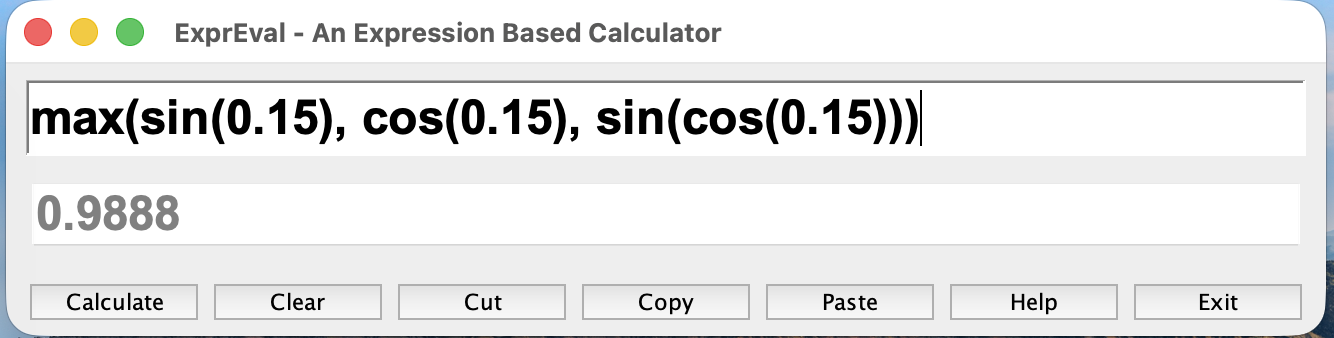
\includegraphics[width=0.7\textwidth]{image/template/test_result/calculate5.png}
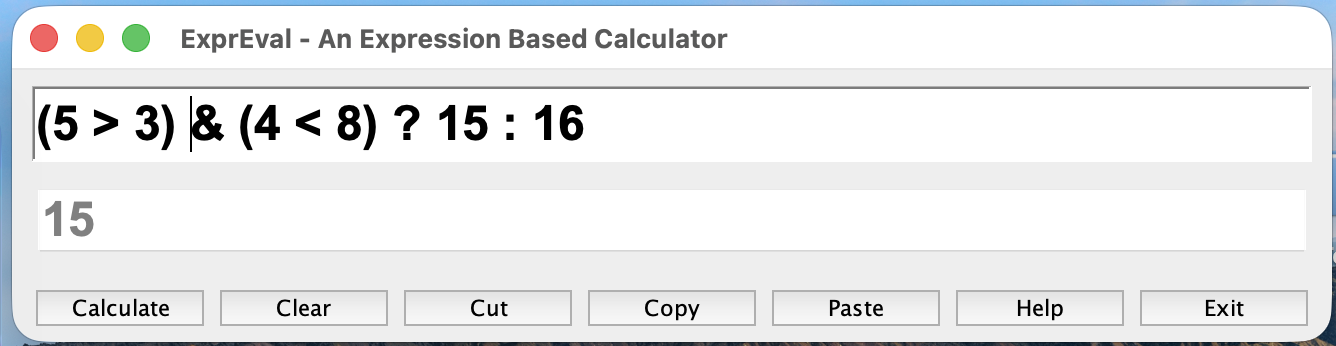
\includegraphics[width=0.7\textwidth]{image/template/test_result/calculate7.png}
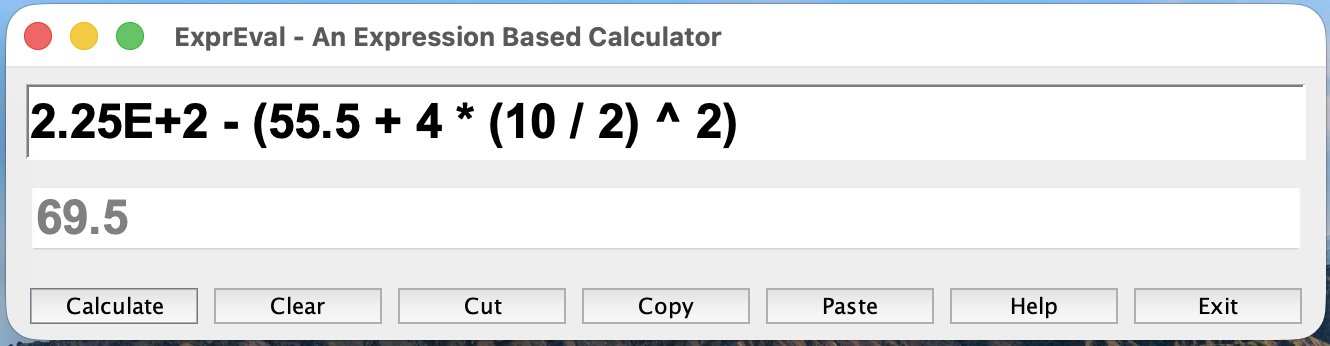
\includegraphics[width=0.7\textwidth]{image/template/test_result/calculate8.png}
\end{figure}

\chapter{自我评分参照}
参照实验规定的记分体系，完成细项列举见表 \ref{tab:self-eval-map}。

\begin{table}[htbp]
    \centering
    \begin{tabular}{|p{5cm}|c|c|}
    \hline
    \textbf{评分项目} & \textbf{权重} & \textbf{对应章节} \\
    \hline
    0. 总分 & 100\% & - \\
    \hline
    1. 基本功能需求 & 55\% & 第 4 章 \\
    1.1 可运行的程序 & 5\% & 4.2 节 \\
    1.2 实验软装置全面测试 & 50\% & 4.1 节 \\
    \hline
    2. 编程风格 & 5\% & 第 3 章 \\
    2.1 标识符命名 & 1\% & 代码 \\
    2.2 文档化注释 & 3\% & 4.4 节 \\
    2.3 程序版面及其他 & 1\% & 代码 \\
    \hline
    3. 面向对象建模与设计 & 15\% & 第 3 章 \\
    3.1 对象属性及其类型设计 & 7\% & 3.3--3.4 节\\
    3.2 对象操作及其接口设计 & 5\% & 3.4 节\\
    3.3 访问控制设计及其他 & 3\% & 3.4 节\\
    \hline
    4. 实验报告 & 25\% & 整篇报告 \\
    4.1 二义性分析 & 2\% & 3.1 节 \\
    4.2 词法分析 & 3\% & 3.2 节 \\
    4.3 算符优先关系表 & 5\% & 3.3 节 \\
    4.4 语法分析与语义处理 & 5\% & 3.4 节 \\
    4.5 实验心得 & 3\% & 第 5 章 \\
    4.6 文档与源程序组织 & 2\% & 第 2 章 \\
    4.7 自定义测试用例 & 5\% & 3.5 节 \\
    \hline
    \end{tabular}
    \caption{评分项目与对应报告章节}
    \label{tab:self-eval-map}
\end{table}


\chapter{实验总结}

\section{技术总结}
本次实验成功地设计并实现了一个完整的基于表达式的计算器 ExprEval。在技术层面，取得了以下核心成果：

\begin{enumerate}
    \item \textbf{完整的词法分析器}：实现了对 Pascal 风格数值常量（含科学记数法）的精确识别，正确处理了各种非法数值形式（如 .11、3.e3、12.3Emax 等）的错误检测，并实现了对布尔常量、预定义函数名的大小写无关识别以及双字符运算符的前瞻匹配。

    \item \textbf{算符优先语法分析器}：构造了覆盖 11 级优先级的算符优先关系表，正确处理了：
    \begin{itemize}
        \item 一元取负（级别 9）与二元减法（级别 6）的重载消歧义；
        \item 幂运算（级别 8）和三元运算（级别 1）的右结合性质；
        \item 预定义函数的可变参数处理与参数个数校验；
        \item 三元运算符的分步归约（? 条件暂存 $\rightarrow$ : 真值暂存 $\rightarrow$ 三元归约）。
    \end{itemize}

    \item \textbf{语义处理程序}：实现了严格的类型推导与兼容性检查。通过 Val 内部类的 isBool 字段标记每个子表达式的类型，确保布尔类型值不会参与算术运算、数值类型值不会被误用于逻辑运算，并正确执行了布尔值不得作为最终计算结果的规定。

    \item \textbf{软件工程实践}：实验结果以100\%正确率通过了已有的测试用例，并且另外编写了 49 个自定义扩展测试用例覆盖规格说明的各类边缘情况，生成 javadoc 文档化注释，编写了跨平台 Makefile 以支持编译、测试、运行和文档生成的自动化。
\end{enumerate}

\section{心得体会}
这次实验让我从零开始完整地经历了编译器前端的设计与实现全过程。在课堂上学习算符优先分析时，我对优先级表、归约动作这些概念停留在理论层面，而亲手实现一个能处理 11 级优先级、涵盖算术/关系/逻辑/三元运算、具有严格类型检查的表达求值器，让我对这一技术有了深刻的理解。

在实现过程中，最有挑战性的部分是三元运算符 ``?:'' 的处理。它分为两个独立的 Token，且处于最低优先级，需要配合辅助栈保存中间状态。调试右结合嵌套时的归约顺序（如 $a\ ?\ b\ ?\ c\ :\ d\ :\ e$）让我切身体会到算符优先分析方法的核心思想：通过优先级决定归约时机，通过结合性决定同级运算符的归约方向。

另外，重载运算符 $-$ 的处理也值得深思。一元取负与二元减法的消歧义完全依赖于语法上下文（当前期望运算量还是运算符），这让我理解了词法分析与语法分析之间的协作关系——词法分析器只负责切分单词，而不判断单词的语法角色，后者交由语法分析器的上下文来完成。

通过这次实验，我对编译原理中词法分析、语法分析和语义处理三个阶段的工程实现有了系统的认识，也对面向对象设计中的封装（将 Lexer、Parser、Evaluator 融合在 Calculator 类中，通过 private 内部类实现信息隐藏）有了更具体的实践体验。

\newclearpage

\backmatter
\makereferences

{
    \appendix
    \chapter{附录代码}
\section{Calculator.java 代码}

\definecolor{codebg}{RGB}{248,249,250}
\definecolor{codeframe}{RGB}{220,223,228}
\definecolor{codekw}{RGB}{25,85,145}
\definecolor{codecm}{RGB}{90,125,90}
\definecolor{codestr}{RGB}{136,44,136}
% Java代码风格
\lstdefinestyle{cleanjava}{
  language=Java,
  basicstyle=\ttfamily\small,
  keywordstyle=\bfseries\color{codekw},
  commentstyle=\itshape\color{codecm},
  stringstyle=\color{codestr},
  backgroundcolor=\color{codebg},
  frame=single,
  rulecolor=\color{codeframe},
  framesep=6pt,
  numbers=left,
  numberstyle=\scriptsize\color{gray},
  numbersep=8pt,
  breaklines=true,
  breakatwhitespace=false,
  showstringspaces=false,
  keepspaces=true,
  tabsize=4,
  columns=fullflexible
}

\lstinputlisting[style=cleanjava,caption={Calculator.java},label={lst:calculator}]{./code/ExprEval/src/parser/Calculator.java}


    \newclearpage
}

\end{document}
